% !TEX root = ../main.tex

\section{Routing incidents taxonomy -- problem definition}
\label{def}
In general, the routing incident is undesirable routing system change, to the state that it is no longer operational or working at suboptimal capacity.



There are several different metrics that can be used to classify routing incident, in this work we will explore criteria/benchmarks such as:
\begin{description}
    \item[\textbf{type}] most important, incident ought to be pinned to a category that ensure unambiguous classification. More on that in \ref{def:tax}
	\item[\textbf{intent}] an incident may originate from intentional, malicious action (so called attack). If done on purpose, possible causes are interception of traffic to espionage, credential theft, censorship or denial of service (downtime, outage) specific website or company. In contrary, erroneous configuration that is result of human mistake, sometimes called \emph{fat finger} mistake, does not have an ultimate agenda.
	\item[\textbf{scale}] the targeted incident might be for one prefix only, but sometimes there will be plenty prefixes involved
	\item[\textbf{impact}] there are multiple factors in this metric, so this will be discussed in \ref{def:impact}
	\item[\textbf{duration}] usually, errors impacting substantial amount of networks or users are corrected in a timely manner, but some small incidents may last weeks unnoticed
	\item[\textbf{range}] some incident will be accepted only by peer AS, but some of them will propagate globally (to the DFZ)
\end{description}

\subsection{Routing incidents characteristics and taxonomy}
\label{def:tax}
The most basic division of routing incidents are \emph{BGP Hijacks} and \emph{Route Leaks}. In this paper we present ... (state of the art/ best in our opinion?) taxonomy. 

\subsubsection{Route leaks}
\label{def:tax:rl}
As defined in \cite{rfc7908}, route leak is propagation of (single or multiple) routing announcement beyond their intended scope, which is defined by routing policy, implemented by a set of redistribution filters. Route leaks are typically not malicious, most often an effect of configuration mistake. 

Most common scenario for leak is when a multihomed stub AS re-advertise a prefix from one of it's transit providers to another. The second provider won't detect a leak and propagate the route further. However, IETF suggest more detailed classification of leaks:

\begin{figure}[ht]
    \begin{center}
   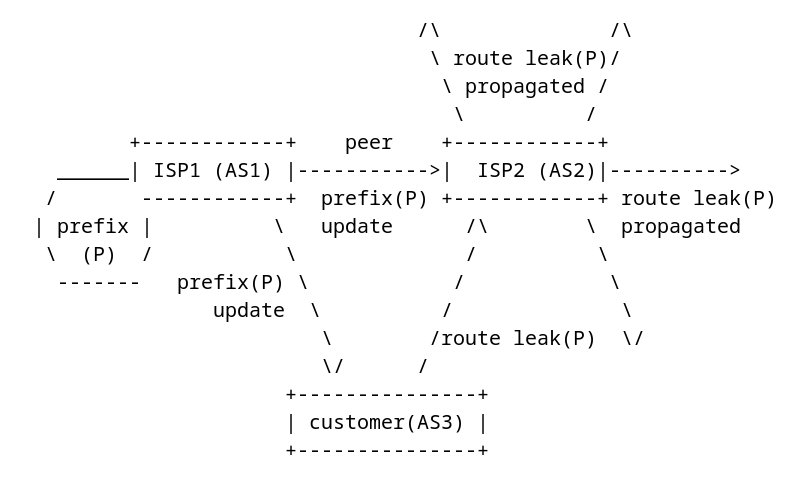
\includegraphics[width = 0.8\linewidth]{./img/route-leak-topology.png}
    \end{center}
    \caption{Route Leak topology \cite{rfc7908} (do przerysowania?) \label{fig:routeleak}}
\end{figure}

\begin{itemize}
    \item \textbf{Type 1: Hairpin Turn with Full Prefix} -- most common case, that makes the stub network that leaked a prefix a transit network. Leak is usually successful, as transit networks usually accept prefixes from their customers. The traffic will reach the destination if stub network will be able to process higher volume of traffic. 
    \item \textbf{Type 2: Lateral ISP-ISP-ISP Leak} -- when ISP's are peering, they should announce only prefixes of their customers. Type 2 takes place when an ISP is propagating prefix of the another ISP whom peering agreement was established.
    \item \textbf{Type 3: Leak of Transit-Provider Prefixes to Peer} -- this type is about propagating prefixes from transit provider to lateral network, effectively providing transit service to the peer.
    \item \textbf{Type 4: Leak of Peer Prefixes to Transit Provider} -- comparing to Type 3, this has the flow in opposite direction . However, it is more dangerous, as it may hurt the peer when the \textsc{AS-Path} is shortened 
    \item \textbf{Type 5: Prefix Re-origination with Data Path to Legitimate Origin} -- offending multihomed AS announces learnt prefix but without original \textsc{AS-Path}. This case is similar to \textbf{Type-0, Exact Prefix, MitM Prefix Hijack} classified in \cite{Sermpezis2018a}, but it assumes that the prefix ought to be learnt from upstream ISP. 
    \item \textbf{Type 6: Accidental Leak of Internal Prefixes and More-Specific Prefixes} -- this type is different, as the prefixes in leak are originating from within offending AS. This is a common issue, typically a badly configured export policy, insufficient aggregation or weak outbound filters. More specific prefixes should not be present in DFZ when a less-specific route exists. In contrast to \textbf{Type-0 Sub-prefix BGP Hijack}, offending AS owns prefixes that are announced.  
\end{itemize}

\subsubsection{BGP Hijacks}
\label{def:tax:hj}
Hijack event is when the adversary Autonomous System illegitimately advertise an IP prefix (or part of it) belonging to other AS. The advertisement needs to propagate towards other BGP speakers if hijack is considered to be successful.

Authors in \cite{Sermpezis2018a} proposed a very detailed taxonomy, with three split categories.  The \emph{affected prefix} can be the same as rightfully originated (\textbf{Exact Prefix Hijack}) or more-specific (\textbf{Sub-Prefix Hijack}), but also not currently advertised (\textbf{Squatting Hijack}) by the victim. Furthermore \emph{AS-Path announced} might be simply substituted for hijacker ASN only (\textbf{Type-0 Hijack}) or modified with victim ASN first and hijacker ASN last in the path (\textbf{Type-N Hijack}). Moreover when the \textsc{AS-Path} is not modified, one should distinguish \textbf{Type-U Hijack}. The third category concerns data-plane traffic handling when a hijack takes place. Possible actions that can be taken by adversary are: \textbf{blackhole} when the traffic is simply dropped, \textbf{man-in-the-middle} for connection eavesdropping or manipulating, or \textbf{imposture} when adversary mimics the victim services and an interaction with legitimate hosts takes place.


%\subsection{Routing incidents characteristics} 

\subsection{Impact of routing incidents}
\label{def:impact}
\subsubsection{BGP Hijacks}
When a Autonomous System attempt Hijack it may affect availability, integrity, and confidentiality of communications in the victim network. The impact depends mostly on the intent of the incident, closely related to the adversary agenda. However, to break down to technical indicators, lets analyse it by the incident type data-plane traffic handling. 

For blackhole there is availability problem for victim's network and possible full outage (denial of service situation). It is similar in effect to data-plane DoS attack, but it's less expected and harder to defend to. 

When considering man-in-the-middle the adversary is creating malicious BGP Hijack it focused on getting the data and keeping the connection intact. Use cases include credential theft, data manipulation .... <TODO>

The most advanced technique is impersonating victim's servers. <TODO>


\subsubsection{Route leaks}
With Route Leaks, <TODO>

Route leak will cause a redirection of traffic to the different path that it was intended. This may or may not result in overloading some network equipment and network links or blackholing the traffic altogether. 

\subsection{Measuring attack impact in the wild}
\label{def:measurement}
Hijacks sometimes have a severe and lasting impact. While it is relatively easy to monitor the state of routing in the Internet's control-plane thanks to initiatives like RIPE RIS\footnote{\url{https://ris-live.ripe.net/}} and software build on top of it or Qrator Radar\footnote{\url{https://radar.qrator.net/}} directly detecting some kind of routing incidents, it is difficult to verify real impact -- users affected and financial losses as companies tend to not disclose such details. 

However, there has been attempt to check real impact of routing incidents. As surveyed among 75 networks from NANOG and RIPE mailing list subscribers in \cite{Sermpezis2018}, 41\% of the operators reported that their organization has been a victim of a hijack in the past. \textquote{The vast majority (76\%) expects the impact of a hijack to last for a long time (few hours or more), while opinions are divided on whether the hijack will affect a few or many of their services/clients, indicating that there are concerns both for extended (e.g.route leaks) and limited/targeted (e.g. malicious attacks) hijacks. (...) More than 57\% of hijacks lasted more than an hour, while 25\% lasted more than a day; around 28\% are short-term hijacks, lasting a few minutes (14.3\%) or seconds (14.3\%). }





\subsection{Incident examples}

MyEtherWallet, provider for Etherum cryptocurrency wallets has been attacked by a BGP hijack on April 24th, 2018\cite{Brandom2018}. The attack was not carried directly at MyEtherWallet, but instead on Amazon Web Services' DNS infrastructure. Worth noting is that AWS DNS was not compromised, but the AWS Route 53 prefix space was the subject of hijack. The resulting outcome was \$365,000 stolen in ETH, in spite of users being warned of self-signed TLS certificate. The attacker was announcing more-specific prefixes (\textbf{sub-prefix hijack}) and running \textbf{man in the middle} proxy for DNS traffic. The cryptocurrency website was \textbf{impersonated}.

Telekom Malaysia (AS4788) and Level3 (AS3549) incident was massive \textbf{Type 4} and \textbf{Type 6} route leak. As described in \cite{Toonk2015}, more than 176 000 prefixes learnt from peering session in DEC-IX and more-specific client prefixes were leaked to upstream provider. This resulted in huge amount of traffic being directed to AS4788 which caused network overload also for Level3. Typical symptoms like packet loss and RTT increase was observed. 

Another case of among many route leak incidents resulted in outage of AWS and Amazon services unavailability. As described by researcher from ThousandEyes in \cite{Kephart2015}, AS33083 announced AWS' prefixes to it's transit provider AS5580. This announcement wasn't in the path before, so the prefix leak is of \textbf{Type 4} \ref{def:tax:rl}. The leak has affected cloud services and therefore multiple companies.





\subsection{Other techniques accompanying routing attacks}
\label{def:mitm}
\subsubsection{Acquisition of Bogus TLS certificate using BGP sub-prefix interception}
Most of the times, to perform a successful attack an adversary is required to do some kind of MiTM attack.
For example, the simplest way to redirect the traffic is to redirect DNS queries and spoof the DNS response.
An attacker will be available to issue a valid TLS certificate, as he will be able to pass all checks that CA is using to verify remote side.
\cite{Gavrichenkov2015}


As presented in \cite{Gavrichenkov2015}, further executed and measured in \cite{BirgeLee2017},\cite{BirgeLee2018}, there is a possibility to issue a valid certificate that should not be issued. The mechanism presented shows a bug in CA's verification procedure, however using BGP routing attack can exploit this bug, leading to further target impersonating by the attacker.
Researchers suggest two countermeasures for CA's: \emph{Multiple Vantage Point Verification} and \emph{Monitoring BGP Route Age}.
